\section{DMA}
\label{zx_next_dma}

% ──────────────────────────────────────────────────────
% ─████████████───██████──────────██████─██████████████─
% ─██░░░░░░░░████─██░░██████████████░░██─██░░░░░░░░░░██─
% ─██░░████░░░░██─██░░░░░░░░░░░░░░░░░░██─██░░██████░░██─
% ─██░░██──██░░██─██░░██████░░██████░░██─██░░██──██░░██─
% ─██░░██──██░░██─██░░██──██░░██──██░░██─██░░██████░░██─
% ─██░░██──██░░██─██░░██──██░░██──██░░██─██░░░░░░░░░░██─
% ─██░░██──██░░██─██░░██──██████──██░░██─██░░██████░░██─
% ─██░░██──██░░██─██░░██──────────██░░██─██░░██──██░░██─
% ─██░░████░░░░██─██░░██──────────██░░██─██░░██──██░░██─
% ─██░░░░░░░░████─██░░██──────────██░░██─██░░██──██░░██─
% ─████████████───██████──────────██████─██████──██████─
% ──────────────────────────────────────────────────────

\input{defines-dma.tex}

The ZX Spectrum Next DMA (zxnDMA) is a single channel direct memory access device that implements a subset of the Z80 DMA functionality. The subset is large enough to be compatible with common uses of the similar Datagear interface available for standard ZX Spectrums but without the idiosyncracies and requirements on the order of commands.

zxnDMA defines two ``ports'', called ``A'' and ``B'' (port is just a word used for referring to both, source and destination). Either one can be used as a source, the other as the destination. They can be memory location or I/O port, auto-increment, auto-decrement or stay fixed. zxnDMA can operate in continuous or burst mode and implements a special feature that can force each byte transfer to take a fixed amount of time, which can be used to deliver sampled audio.


\subsection{Programming}

% note: since both ports are declared on the same page, we only link to the page once
Since core 3.1.2, zxnDMA is mapped to \PortTextXRef[]{xx6B} and legacy Zilog DMA to \PortTextXRef[]{xx0B} (see page \PortPage{xx0B} for details).

Similar to Z80 DMA, zxnDMA also has 7 write registers named \DMARegName{WR0}-\DMARegName{WR6}. Some of the bits are used to identify a register, while the rest represent the payload ({\tt x} in the table below):

% Registers are defined with specific bit configuration ({\tt 0} or {\tt 1} in the table below) while the rest of the bits define the payload ({\tt x}):

\begin{ElegantTableX}{|l|l|X|}[
	\newcommand{\DMAReg}[3]{{\tt #1} & {\tt #2} & #3 \\}
]

	\ElegantHeader{
		\EH{Reg.} & \EH{Bitmask} & \EH{Description}
	}

	\DMAReg{WR0}{0xxxxx01}{Direction, operation and port A configuration}
	\hline

	\DMAReg{WR1}{0xxxx100}{Port A configuration}
	\hline

	\DMAReg{WR2}{0xxxx000}{Port B configuration}
	\hline

	\DMAReg{WR3}{1xxxxx00}{Activation}
	\hline

	\DMAReg{WR4}{1xxxxx01}{Port B, timing and interrupt configuration}
	\hline

	\DMAReg{WR5}{10xxx010}{Ready and stop configuration}
	\hline

	\DMAReg{WR6}{1xxxxx11}{Command register}

\end{ElegantTableX}

Each register can include zero or more parameters. Most often specific bits in the payload define whether and which parameters are used. Each parameter is one byte long. Parameters are written immediately after the base register byte. If multiple parameters are used, the order is specified by the bit position within the base payload. The order is from right to left, the parameter associated with bit {\tt 0} is written first, the one from bit {\tt 7} last.

Sometimes it's also possible that a specific configuration of parameter byte requires additional bytes to be inserted. If so, these bytes are inserted immediately after their ``parent'' parameter byte following the same rules as indicated above. Only after all child parameters are written, we continue with other parents' parameters, if there are more. This forms a sort of recursive pattern.

After all parameters are written, we can start with a new register byte again. This is then repeated until zxnDMA program is started using \DMARegName{WR3} or (preferably) \DMARegName{WR6}. The same registers can be repeated multiple times within the same DMA program.

DMA programs can be up to 256 bytes long (but the data being transferred can be up to 64K).


\pagebreak
\subsection{Registers at a Glance}

\begin{multicols}{2}
	
	\DMAScaledReg{WR0}{
		\begin{tikzpicture}

			% Instruction Byte
			\DMABitHeader
			\DMABitValue{7}{0}
			\DMABitValue{6}{}
			\DMABitValue{5}{}
			\DMABitValue{4}{}
			\DMABitValue{3}{}
			\DMABitValue{2}{}
			\DMABitValue{1}{0}
			\DMABitValue{0}{1}
		
			% Bit 2 description
			\DMABitDescTitle{2}{Transfer Direction}
			\DMABitDescItem{2}{0}{Port B$\rightarrow$A}
			\DMABitDescItem{2}{1}{Port A$\rightarrow$B}
		
			% Parameters
			\DMABitPar{3}{Port A address (LSB)}[1ex][pos=0.35][]
			\DMABitPar{4}{Port A address (MSB)}[][pos=0.35][]
			\DMABitPar{5}{Block length (LSB)}[][pos=0.35][]
			\DMABitPar{6}{Block length (MSB)}[][pos=0.35][]
		
		\end{tikzpicture}
	}

	\DMAScaledReg{WR1}{
		\begin{tikzpicture}
	
			% Instruction Byte
			\DMABitHeader
			\DMABitValue{7}{0}
			\DMABitValue{6}{}
			\DMABitValue[2]{5}{}
			\DMABitValue{3}{}
			\DMABitValue{2}{1}
			\DMABitValue{1}{0}
			\DMABitValue{0}{0}
	
			% Bit 3 description
			\DMABitDescTitle{3}{Port A Source}
			\DMABitDescItem{3}{0}{Port A is Memory}
			\DMABitDescItem{3}{1}{Port A is I/O}
	
			% Bit 5-4 description
			\DMABitDescTitle[-3ex]{5}{Port A Address Handling}
			\DMABitDescItem{5}{\DMATwoBits{0}{0}}{Port A Address Decrements}
			\DMABitDescItem{5}{\DMATwoBits{0}{1}}{Port A Address Increments}
			\DMABitDescItem{5}{\DMATwoBits{1}{0}}{Port A Address is Fixed}
			\DMABitDescItem{5}{\DMATwoBits{1}{1}}{Port A Address is Fixed}
		
			% Parameters
			\DMABitParHeader{6}{Port A Timing}[]
			\DMABitValue{7}{0}
			\DMABitValue{6}{0}
			\DMABitValue{5}{0}
			\DMABitValue{4}{0}
			\DMABitValue{3}{0}
			\DMABitValue{2}{0}
			\DMABitValue[2]{1}{}
		
			% Par bit 1-0 description
			\DMABitDescTitle[-3ex]{1}{Port A Variable Timing}
			\DMABitDescItem{1}{\DMATwoBits{0}{0}}{Cycle length = 4}
			\DMABitDescItem{1}{\DMATwoBits{0}{1}}{Cycle length = 3}
			\DMABitDescItem{1}{\DMATwoBits{1}{0}}{Cycle length = 2}
			\DMABitDescItem{1}{\DMATwoBits{1}{1}}{Do not use!}
	
		\end{tikzpicture}
	}

	\DMAScaledReg{WR2}{
		\begin{tikzpicture}
	
			% Instruction Byte
			\DMABitHeader
			\DMABitValue{7}{0}
			\DMABitValue{6}{}
			\DMABitValue[2]{5}{}
			\DMABitValue{3}{}
			\DMABitValue{2}{0}
			\DMABitValue{1}{0}
			\DMABitValue{0}{0}

			% Bit 3 description
			\DMABitDescTitle{3}{Port B source}
			\DMABitDescItem{3}{0}{Port B is Memory}
			\DMABitDescItem{3}{1}{Port B is I/O}

			% Bit 5-4 description
			\DMABitDescTitle[-3ex]{5}{Port B Address Handling}
			\DMABitDescItem{5}{\DMATwoBits{0}{0}}{Port B Address Decrements}
			\DMABitDescItem{5}{\DMATwoBits{0}{1}}{Port B Address Increments}
			\DMABitDescItem{5}{\DMATwoBits{1}{0}}{Port B Address is Fixed}
			\DMABitDescItem{5}{\DMATwoBits{1}{1}}{Port B Address is Fixed}
	
			% Parameter 1
			\DMABitParHeader{6}{Port B Timing}[]
			\DMABitValue{7}{0}
			\DMABitValue{6}{0}
			\DMABitValue{5}{}
			\DMABitValue{4}{0}
			\DMABitValue{3}{0}
			\DMABitValue{2}{0}
			\DMABitValue[2]{1}{}
	
			% Parameter 1 bit 1-0 description
			\DMABitDescTitle[-3ex]{1}{Port B Variable Timing}
			\DMABitDescItem{1}{\DMATwoBits{0}{0}}{Cycle Length = 4}
			\DMABitDescItem{1}{\DMATwoBits{0}{1}}{Cycle Length = 3}
			\DMABitDescItem{1}{\DMATwoBits{1}{0}}{Cycle Length = 2}
			\DMABitDescItem{1}{\DMATwoBits{1}{1}}{Do not use!}
	
			% Parameter 2
			\DMABitPar{5}{Prescalar (Fixed Time Transfer)}[1ex][near start][]

		\end{tikzpicture}
	}

	\columnbreak

	\DMAScaledReg{WR3}{
		\begin{tikzpicture}
	
			% Instruction Byte
			\DMABitHeader
			\DMABitValue{7}{1}
			\DMABitValue{6}{}
			\DMABitValue{5}{0}
			\DMABitValue{4}{0}
			\DMABitValue{3}{0}
			\DMABitValue{2}{0}
			\DMABitValue{1}{0}
			\DMABitValue{0}{0}

			% Bit 3 description
			\DMABitDescTitle{6}{Activation}
			\DMABitDescItem{6}{0}{DMA Disabled}
			\DMABitDescItem{6}{1}{DMA Enabled}
	
		\end{tikzpicture}
	}

	\DMAScaledReg{WR4}{
		\begin{tikzpicture}

			\pgfdeclarelayer{above}
			\pgfsetlayers{main,above}
	
			% Instruction Byte
			\DMABitHeader
			\DMABitValue{7}{1}
			\DMABitValue[2]{6}{}
			\DMABitValue{4}{0}
			\DMABitValue{3}{}
			\DMABitValue{2}{}
			\DMABitValue{1}{0}
			\DMABitValue{0}{1}

			% Bit 6 description
			\begin{pgfonlayer}{above}
				% we only need fill on top of text to avoid lines drawn on top. Coordinates were set via trial & error, so any change in data will also require re-positioning...
				\node[fill=white, opacity=0.95, minimum width=3em, minimum height=5.7em] at(2.5,-2.4) {};

				\DMABitDescTitle{6}{DMA Mode}
				\DMABitDescItem{6}{\DMATwoBits{0}{0}}{Do not use!}
				\DMABitDescItem{6}{\DMATwoBits{0}{1}}{Continuous Mode}
				\DMABitDescItem{6}{\DMATwoBits{1}{0}}{Burst Mode}
				\DMABitDescItem{6}{\DMATwoBits{1}{1}}{Do not use!}
			\end{pgfonlayer}
	
			% Parameters
			\DMABitPar{2}{Port B Address (LSB)}[1ex][pos=0.2][]
			\DMABitPar{3}{Port B Address (MSB)}[][pos=0.2][]

		\end{tikzpicture}
	}

	\DMAScaledReg{WR5}{
		\begin{tikzpicture}
	
			% Instruction Byte
			\DMABitHeader
			\DMABitValue{7}{1}
			\DMABitValue{6}{0}
			\DMABitValue{5}{}
			\DMABitValue{4}{}
			\DMABitValue{3}{0}
			\DMABitValue{2}{0}
			\DMABitValue{1}{1}
			\DMABitValue{0}{0}

			% Bit 4 description
			\DMABitDescTitle{4}{Ready Configuration}
			\DMABitDescItem{4}{0}{\DMAPinLabel{CE} only}
			\DMABitDescItem{4}{1}{\DMAPinLabel{CE} and \DMAPinLabel{}{WAIT} multiplexed}
	
			% Bit 5 description
			\DMABitDescTitle{5}{Stop Configuration}
			\DMABitDescItem{5}{0}{Stop on End of Block}
			\DMABitDescItem{5}{1}{Auto Restart on End of Block}
	
		\end{tikzpicture}
	}

	\DMAScaledReg{WR6}{
		\begin{tikzpicture}
	
			\newcommand{\DMAWRBits}[5]{#1\hspace*{1.8ex}#2\hspace*{1.8ex}#3\hspace*{1.8ex}#4\hspace*{1.8ex}#5}
			\newcommand{\DMAWRHex}[2]{\MemAddr{#1}\hspace*{1.8ex}#2}
		
			% Instruction Byte
			\DMABitHeader
			\DMABitValue{7}{1}
			\DMABitValue[5]{6}{}
			\DMABitValue{1}{1}
			\DMABitValue{0}{1}
	
			% Bit 6-2 description
			\DMABitDescTitle[-7.5ex]{6}{Command}
			\DMABitDescItem{6}{\DMAWRBits{0}{0}{0}{0}{1}}{\DMAWRHex{87}{Enable DMA}}
			\DMABitDescItem{6}{\DMAWRBits{0}{0}{0}{0}{0}}{\DMAWRHex{83}{Disable DMA}}
			\DMABitDescItem{6}{\DMAWRBits{0}{0}{0}{1}{0}}{\DMAWRHex{8B}{Reinitialize Status Byte}}
			\DMABitDescItem{6}{\DMAWRBits{0}{1}{0}{0}{1}}{\DMAWRHex{A7}{Initialize Read Sequence}}
			\DMABitDescItem{6}{\DMAWRBits{0}{1}{1}{0}{0}}{\DMAWRHex{B3}{Force Ready}}
			\DMABitDescItem{6}{\DMAWRBits{0}{1}{1}{1}{0}}{\DMAWRHex{BB}{Read Mask Follows (see below)}}
			\DMABitDescItem{6}{\DMAWRBits{0}{1}{1}{1}{1}}{\DMAWRHex{BF}{Read Status Byte}}
			\DMABitDescItem{6}{\DMAWRBits{1}{0}{0}{0}{0}}{\DMAWRHex{C3}{Reset}}
			\DMABitDescItem{6}{\DMAWRBits{1}{0}{0}{0}{1}}{\DMAWRHex{C7}{Reset Port A Timing}}
			\DMABitDescItem{6}{\DMAWRBits{1}{0}{0}{1}{0}}{\DMAWRHex{CB}{Reset Port B Timing}}
			\DMABitDescItem{6}{\DMAWRBits{1}{0}{0}{1}{1}}{\DMAWRHex{CF}{Load}}
			\DMABitDescItem{6}{\DMAWRBits{1}{0}{1}{0}{0}}{\DMAWRHex{D3}{Continue}}
		
			% Parameter
			\DMABitParHeader{}{Read Mask}[]
			\DMABitValue{7}{1}
			\DMABitValue{6}{}
			\DMABitValue{5}{}
			\DMABitValue{4}{}
			\DMABitValue{3}{}
			\DMABitValue{2}{}
			\DMABitValue{1}{}
			\DMABitValue{0}{}
		
			% Read bytes
			\DMABitPar{0}{Status}[1em][pos=0.5][]
			\DMABitPar{1}{Byte Counter LSB}[][pos=0.37][]
			\DMABitPar{2}{Byte Counter MSB}[][pos=0.30][]
			\DMABitPar{3}{Port A Address LSB}[][pos=0.26][]
			\DMABitPar{4}{Port A Address MSB}[][pos=0.23][]
			\DMABitPar{5}{Port B Address LSB}[][pos=0.21][]
			\DMABitPar{6}{Port B Address MSB}[][pos=0.2][]
		
		\end{tikzpicture}
	}
	
\end{multicols}


\pagebreak
\subsection{WR0 - Direction, Operation, Port A Configuration}

% ▒█░░▒█ ▒█▀▀█ █▀▀█ 
% ▒█▒█▒█ ▒█▄▄▀ █▄▀█ 
% ▒█▄▀▄█ ▒█░▒█ █▄▄█

\DMARegName{WR0} specifies the direction of the transfer, the length of the data that will be transferred and port A address. Base register byte can be followed by up to four parameter bytes:

\begin{tikzpicture}

	% Instruction Byte
	\DMABitHeader
	\DMABitValue{7}{0}
	\DMABitValue{6}{}
	\DMABitValue{5}{}
	\DMABitValue{4}{}
	\DMABitValue{3}{}
	\DMABitValue{2}{}
	\DMABitValue[2]{1}{}

	% Bits 1-0 description
	\DMABitDescTitle[-3ex]{1}{Operation}
	\DMABitDescItem{1}{\DMATwoBits{0}{0}}{Do not use! {\small (Reserved for {\tt WR1} and {\tt WR2})}}
	\DMABitDescItem{1}{\DMATwoBits{0}{1}}{Transfer}
	\DMABitDescItem{1}{\DMATwoBits{1}{0}}{Do not use! {\small (Behaves like transfer)}}
	\DMABitDescItem{1}{\DMATwoBits{1}{1}}{Do not use! {\small (Behaves like transfer)}}

	% Bit 2 description
	\DMABitDescTitle{2}{Transfer Direction}
	\DMABitDescItem{2}{0}{Port B$\rightarrow$A}
	\DMABitDescItem{2}{1}{Port A$\rightarrow$B}

	% Parameters
	\DMABitPar{3}{Port A starting address (LSB)}[1ex][pos=0.35]
	\DMABitPar{4}{Port A starting address (MSB)}[][pos=0.35]
	\DMABitPar{5}{Block length (LSB)}[][pos=0.35]
	\DMABitPar{6}{Block length (MSB)}[][pos=0.35]

	% Legend
	\DMALegend{\DMABitParID{3}}

\end{tikzpicture}


\subsubsection{Base Register Byte}

\begin{DMADescription}

	\DMADescriptionItem{1-0}{Operation}{
		The combination of these two bits defines the type of operation the DMA program will use. While all four combinations are listed, zxnDMA only supports one at the moment - {\tt 01}:

		\begin{DMAList}
			\item[{\tt 00}] Don't use, it conflicts with \DMARegName{WR1} and \DMARegName{WR2}.
			
			\item[{\tt 01}] Transfer; this is the only supported operation on zxnDMA.
			
			\item[{\tt 10}] Not recommended for compatibility reasons: at the moment {\tt 10} behaves exactly like {\tt 01} (transfer) on zxnDMA, but on Z80 it's ``search'' instead. So there is a possibility this will change in future cores.
			
			\item[{\tt 11}] Similar to {\tt 10}; at the moment it behaves like {\tt 01} (transfer) on zxnDMA, but on Z80 it's ``search/transfer''. Again, this may change in future cores.
		\end{DMAList}
	}

	\DMADescriptionItem{2}{Transfer Direction}{
		Provides the destination of the data transfer:

		\begin{DMAList}
			\item[{\tt 0}] Port B is source, port A destination.
			\item[{\tt 1}] Port A is source, port B destination.
		\end{DMAList}

		Either port can act as source, while the other becomes the destination.
	}

	\DMADescriptionItem{4-3}{Port A Starting Address}{
		Regardless of whether port A acts as a source or destination, we have to define its source address. To do so, set both bits to {\tt 1}. The address is then entered immediately after this byte. The address is interpreted either as memory or I/O port, based on the configuration from \DMARegName{WR1}.
	}

	\DMADescriptionItem{6-5}{Transfer Length}{
		All DMA operations must have a length defined. Therefore this parameter is also required - set both bits to {\tt 1}. The length is a 16-bit value and needs to be entered at the end of the data for \DMARegName{WR0} register.
	}

\end{DMADescription}


\subsubsection{Port A Starting Address}

If bit 3 of the base register byte is set, then LSB of port A starting address is expected as the first parameter after the base. If bit 4 is set, then MSB byte is expected. If both bits are set, then LSB needs to be written first, followed by MSB. This is in fact the most common setup because port A starting address is required for each DMA operation. And since little-endian format is used, the value forming the 16-bit starting address of port A can be written directly. For example:

\begin{tcblisting}{}
	DW &253B          ; Port A starts at &253B
\end{tcblisting}
\vspace*{-1ex}

Or, if we have a label that points to the start of the memory:

\begin{tcblisting}{}
	DW StartLabel     ; Port A starts on memory at this label
\end{tcblisting}
\vspace*{-1ex}

Whether the address represents a memory location or I/O port is defined with \DMARegName{WR1}.


\subsubsection{Transfer Length}{

Setting bit 5 of the base register byte is associated with LSB of transfer length and bit 6 with MSB. If both bits are set, which is the usual case, then LSB is written first, followed by MSB. Again, 16-bit length can be written directly in this case, as shown above with port A starting address.


\subsubsection{Notes}

Since all parameters in \DMARegName{WR0} are important for DMA transfer, they are typically always included. The configuration would most often look something like this:

\begin{tcblisting}{}
	DB %01111101      ; WR0 - append length and port A address, A->B
	DW &253B          ; Port A starts at &253B
	DW 1500           ; We will transfer 1500 bytes
\end{tcblisting}

Usually, the address and length are provided dynamically, and frequently ``self-modifying code'' approach is used to fill this data on the fly. We'll discuss this in the example section later on.



\pagebreak
\subsection{WR1 - Port A Configuration}

% ▒█░░▒█ ▒█▀▀█ ▄█░ 
% ▒█▒█▒█ ▒█▄▄▀ ░█░ 
% ▒█▄▀▄█ ▒█░▒█ ▄█▄"

This is where we provide details about port A. Base register byte may be followed by one parameter, if bit 6 of the base byte is set:

\begin{tikzpicture}
	
	% Instruction Byte
	\DMABitHeader
	\DMABitValue{7}{0}
	\DMABitValue{6}{}
	\DMABitValue[2]{5}{}
	\DMABitValue{3}{}
	\DMABitValue{2}{1}
	\DMABitValue{1}{0}
	\DMABitValue{0}{0}

	% Bit 3 description
	\DMABitDescTitle{3}{Port A Source}
	\DMABitDescItem{3}{0}{Port A is Memory}
	\DMABitDescItem{3}{1}{Port A is I/O}

	% Bit 5-4 description
	\DMABitDescTitle[-3ex]{5}{Port A Address Handling}
	\DMABitDescItem{5}{\DMATwoBits{0}{0}}{Port A Address Decrements}
	\DMABitDescItem{5}{\DMATwoBits{0}{1}}{Port A Address Increments}
	\DMABitDescItem{5}{\DMATwoBits{1}{0}}{Port A Address is Fixed}
	\DMABitDescItem{5}{\DMATwoBits{1}{1}}{Port A Address is Fixed}
	
	% Parameters
	\DMABitParHeader{6}{Port A Timing}
	\DMABitValue{7}{0}
	\DMABitValue{6}{0}
	\DMABitValue{5}{0}
	\DMABitValue{4}{0}
	\DMABitValue{3}{0}
	\DMABitValue{2}{0}
	\DMABitValue[2]{1}{}
	
	% Par bit 1-0 description
	\DMABitDescTitle[-3ex]{1}{Port A Variable Timing}
	\DMABitDescItem{1}{\DMATwoBits{0}{0}}{Cycle length = 4}
	\DMABitDescItem{1}{\DMATwoBits{0}{1}}{Cycle length = 3}
	\DMABitDescItem{1}{\DMATwoBits{1}{0}}{Cycle length = 2}
	\DMABitDescItem{1}{\DMATwoBits{1}{1}}{Do not use!}

	% Legend
	\DMALegend{\DMABitDefID{7}}[PARAMETER]

\end{tikzpicture}

\subsubsection{Base Register Byte}

\begin{DMADescription}
	
	\DMADescriptionItem{3}{Port A Source}{
		Specifies the type of the address for port A (the address is written with \DMARegName{WR0}):

		\begin{DMAList}
			\item[{\tt 0}] Port A address is memory location.
			\item[{\tt 1}] Port A address is I/O port.
		\end{DMAList}
	}

	\DMADescriptionItem{5-4}{Port A Address Handling}{
		The combination of these two bits determines how port A address will be handled after each byte is transferred:

		\begin{DMAList}
			\item[{\tt 00}] Address is decremented after byte is transferred.
			
			\item[{\tt 01}] Address is incremented after byte is transferred.
				
			\item[{\tt 10}] The address remains fixed at its starting value. This is typically used when port A is an I/O port; all bytes are sent to the same port in this case.
				
			\item[{\tt 11}] The same as {\tt 10}, address is fixed.
		\end{DMAList}

		In case of decrementing or incrementing, the first byte is read from or written to the starting address for port A from \DMARegName{WR0}, then decrementing or incrementing begins for the second and subsequent bytes.
	}

	\DMADescriptionItem{6}{Port A Timing}{
		If bit 6 is set, the next byte written to the DMA after \DMARegName{WR1} base register byte is used to define port A variable timing. If bit 6 is {\tt 0}, standard Z80 timing for read and write cycles is used.
	}

\end{DMADescription}


\pagebreak
\subsubsection{Port A Timing}

This byte is expected if bit 6 of the base register byte is set. Only bits 1 and 0 are used, the rest must be set to {\tt 0}.

\begin{DMADescription}
	
	\DMADescriptionItem{1-0}{Port A Timing}{
		Specifies variable timing configuration for port A that allows shortening the length of port A read or write cycles:

		\begin{DMAList}
			\item[{\tt 00}] Cycle length is 4.
			\item[{\tt 01}] Cycle length is 3.
			\item[{\tt 10}] Cycle length is 2.
			\item[{\tt 11}] Do not use!
		\end{DMAList}

		The cycle lengths are intended to selectively slow down read or write cycles for hardware that can't operate at the DMA full speed.
	}

\end{DMADescription}

In contrast with Z80 DMA, zxnDMA doesn't support half-cycle timing for control signals.


\pagebreak
\subsection{WR2 - Port B Configuration}

% ▒█░░▒█ ▒█▀▀█ █▀█ 
% ▒█▒█▒█ ▒█▄▄▀ ░▄▀ 
% ▒█▄▀▄█ ▒█░▒█ █▄▄

This register is similar to \DMARegName{WR1} except it sets the configuration for port B. If bit 6 is set, base register byte needs to be followed by one parameter. And the configuration of this parameter may in turn require one more parameter byte to be appended.

\begin{tikzpicture}
	
	% Instruction Byte
	\DMABitHeader
	\DMABitValue{7}{0}
	\DMABitValue{6}{}
	\DMABitValue[2]{5}{}
	\DMABitValue{3}{}
	\DMABitValue{2}{0}
	\DMABitValue{1}{0}
	\DMABitValue{0}{0}

	% Bit 3 description
	\DMABitDescTitle{3}{Port B source}
	\DMABitDescItem{3}{0}{Port B is Memory}
	\DMABitDescItem{3}{1}{Port B is I/O}

	% Bit 5-4 description
	\DMABitDescTitle[-3ex]{5}{Port B Address Handling}
	\DMABitDescItem{5}{\DMATwoBits{0}{0}}{Port B Address Decrements}
	\DMABitDescItem{5}{\DMATwoBits{0}{1}}{Port B Address Increments}
	\DMABitDescItem{5}{\DMATwoBits{1}{0}}{Port B Address is Fixed}
	\DMABitDescItem{5}{\DMATwoBits{1}{1}}{Port B Address is Fixed}
	
	% Parameter 1
	\DMABitParHeader{6}{Port B Timing}
	\DMABitValue{7}{0}
	\DMABitValue{6}{0}
	\DMABitValue{5}{}
	\DMABitValue{4}{0}
	\DMABitValue{3}{0}
	\DMABitValue{2}{0}
	\DMABitValue[2]{1}{}
	
	% Parameter 1 bit 1-0 description
	\DMABitDescTitle[-3ex]{1}{Port B Variable Timing}
	\DMABitDescItem{1}{\DMATwoBits{0}{0}}{Cycle Length = 4}
	\DMABitDescItem{1}{\DMATwoBits{0}{1}}{Cycle Length = 3}
	\DMABitDescItem{1}{\DMATwoBits{1}{0}}{Cycle Length = 2}
	\DMABitDescItem{1}{\DMATwoBits{1}{1}}{Do not use!}
	
	% Parameter 2
	\DMABitPar{5}{Prescalar (Fixed Time Transfer)}

	% Legend
	\DMALegend{\DMABitDefAnyID{1}{7}}

\end{tikzpicture}

\subsubsection{Base Register Byte}

\begin{DMADescription}

	\DMADescriptionItem{3}{Port B\\Source}{
		Specifies the type of the address for port B (the address is written with \DMARegName{WR4}):

		\begin{DMAList}
			\item[{\tt 0}] Port B address is memory location.
			\item[{\tt 1}] Port B address is I/O port.
		\end{DMAList}
	}

	\DMADescriptionItem{5-4}{Port B Address Handling}{
		The combination of the two bits determines how port B address will be handled after each byte is transferred:
	
		\begin{DMAList}
			\item[{\tt 00}] Address is decremented after byte is transferred.
				
			\item[{\tt 01}] Address is incremented after byte is transferred.
					
			\item[{\tt 10}] The address remains fixed at its starting value. This is typically used when port B is an I/O port; all bytes are sent to the same port in this case.
					
			\item[{\tt 11}] The same as {\tt 10}, address is fixed.
		\end{DMAList}
	
		In case of decrementing or incrementing, the first byte is read from or written to the starting address for port B from \DMARegName{WR4}, then decrementing or incrementing begins for the second and subsequent bytes.
	}
	
	\DMADescriptionItem{6}{Port B Timing}{
		If bit 6 is set, the next byte written to the DMA after \DMARegName{WR2} base register byte is used to define port B variable timing. If bit 6 is {\tt 0}, standard Z80 timing for read and write cycles is used.
	}

\end{DMADescription}


\subsubsection{Port B Timing}

This byte is expected if bit 6 of the base register byte is set. Only bits 5, 1 and 0 are used, the rest must be set to {\tt 0}.

\begin{DMADescription}
	
	\DMADescriptionItem{1-0}{Port A Timing}{
		Specifies variable timing configuration for port A that allows shortening the length of port A read or write cycles:

		\begin{DMAList}
			\item[{\tt 00}] Cycle length is 4.
			\item[{\tt 01}] Cycle length is 3.
			\item[{\tt 10}] Cycle length is 2.
			\item[{\tt 11}] Do not use!
		\end{DMAList}

		The cycle lengths are intended to selectively slow down read or write cycles for hardware that can't operate at the DMA full speed.
	}

	\DMADescriptionItem{5}{Enable Prescalar}{
		If set, then additional byte is expected with prescalar value used for fixed time transfers. See below for details.
	}

\end{DMADescription}

In contrast with Z80 DMA, zxnDMA doesn't support half-cycle timing for control signals.


\subsubsection{Prescalar - Fixed Time Transfer}

This byte is expected if bit 5 of ``Port B Timing'' is set. This is a feature of zxnDMA not present in Z80. If non-zero value is written, a delay will be inserted after each byte is transferred. The delay is calculated so that the total amount of time for each byte, including time required for actual transfer, is determined by the prescalar value.

To calculate prescalar value, use formula: $prescalar = 875kHz / rate$ where rate is desired frequency. For example to have a constant rate of 16kHz, prescalar needs to be set to 55 (calculation gives 54.6875 which needs to be rounded). The constant 875kHz is assumed for 28MHz system clock. But exact system clock depends on video timing selected by user (HDMI, VGA). The actual value should therefore be adjusted according to exact frequency as described with \PortTextXRef{11}.

Fixed time transfer works in continuous and burst mode (see \DMARegName{WR4}). In burst mode, DMA will give up any waiting time to the CPU so it can run while DMA is idle.


\pagebreak
\subsection{WR3 - Activation}

% ▒█░░▒█ ▒█▀▀█ █▀▀█ 
% ▒█▒█▒█ ▒█▄▄▀ ░░▀▄ 
% ▒█▄▀▄█ ▒█░▒█ █▄▄█

Compared to Z80 DMA, Next only uses one bit:

\begin{tikzpicture}
	
	% Instruction Byte
	\DMABitHeader
	\DMABitValue{7}{1}
	\DMABitValue{6}{}
	\DMABitValue{5}{0}
	\DMABitValue{4}{0}
	\DMABitValue{3}{0}
	\DMABitValue{2}{0}
	\DMABitValue{1}{0}
	\DMABitValue{0}{0}

	% Bit 3 description
	\DMABitDescTitle{6}{Activation}
	\DMABitDescItem{6}{0}{DMA Disabled}
	\DMABitDescItem{6}{1}{DMA Enabled}
	
\end{tikzpicture}


\subsubsection{Base Register Byte}

\begin{DMADescription}
	
	\DMADescriptionItem{6}{Enable\\DMA}{
		If set, DMA will be enabled, otherwise disabled. DMA should be enabled only after all other bytes are written.

		Note: while enabling/disabling through \DMARegName{WR3} works on Next, it's recommended to use \DMARegName{WR6} instead.
	}

\end{DMADescription}

\subsection{WR4 - Port B, Timing, Interrupt Control}

% ▒█░░▒█ ▒█▀▀█ ░█▀█░ 
% ▒█▒█▒█ ▒█▄▄▀ █▄▄█▄ 
% ▒█▄▀▄█ ▒█░▒█ ░░░█░

Another register where zxnDMA uses only a small portion of functionality from Z80 DMA:

\begin{tikzpicture}

	\pgfdeclarelayer{above}
	\pgfsetlayers{main,above}
	
	% Instruction Byte
	\DMABitHeader
	\DMABitValue{7}{1}
	\DMABitValue[2]{6}{}
	\DMABitValue{4}{0}
	\DMABitValue{3}{}
	\DMABitValue{2}{}
	\DMABitValue{1}{0}
	\DMABitValue{0}{1}

	% Bit 6 description
	\begin{pgfonlayer}{above}
		% we only need fill on top of text to avoid lines drawn on top. Coordinates were set via trial & error, so any change in data will also require re-positioning...
		\node[fill=white, opacity=0.95, minimum width=3em, minimum height=5.2em] at(2.5,-3.1) {};

		\DMABitDescTitle[-3ex]{6}{DMA Mode}[2.5em]
		\DMABitDescItem{6}{\DMATwoBits{0}{0}}{Do not use! {\small (Behaves like continuous mode)}}
		\DMABitDescItem{6}{\DMATwoBits{0}{1}}{Continuous Mode}
		\DMABitDescItem{6}{\DMATwoBits{1}{0}}{Burst Mode}
		\DMABitDescItem{6}{\DMATwoBits{1}{1}}{Do not use!}
	\end{pgfonlayer}
	
	% Parameters
	\DMABitPar{2}{Port B Starting Address (LSB)}[1ex][pos=0.2]
	\DMABitPar{3}{Port B Starting Address (MSB)}[][pos=0.2]

	% Legend
	\DMALegend{\DMABitParID{2}}[PARAMS]

\end{tikzpicture}


\subsubsection{Base Register Byte}

\begin{DMADescription}

	\DMADescriptionItem{3-2}{Port B Starting Address}{
		Similar to bits 4-3 of \DMARegName{WR0}, these two bits indicate that port B address will follow. Bit 3 enables LSB and bit 2 MSB of the address. Each byte can be enabled separately, though most commonly, both are used. The address is interpreted either as memory or I/O port, based on the configuration from \DMARegName{WR2}.
	}
	
	\DMADescriptionItem{6-5}{DMA Mode}{
		Specifes operating mode for DMA:
	
		\begin{DMAList}
			\item[{\tt 00}] Not recommended for compatibility reasons: at the moment {\tt 00} behaves exactly like {\tt 01} (continuous mode) on zxnDMA, but on Z80 it's ``byte'' mode. So there is a possibility this will change in future cores.
				
			\item[{\tt 01}] Continuous mode. When the CPU starts DMA, it will run to completion without allowing the CPU to run. The CPU will only execute the next instruction after DMA completes.
				
			\item[{\tt 10}] Burst mode. In this mode, DMA will let the CPU run if either port is not ready. With zxnDMA, this condition can only occur when operating in fixed time transfer mode, as described with \DMARegName{WR2}.
				
			\item[{\tt 11}] Do not use!
		\end{DMAList}
	}
	
\end{DMADescription}


\subsubsection{Port B Starting Address}

This works exactly the same as port A starting address in bits 4-3 of \DMARegName{WR0}, but for port B. Bit 3 of base register enables LSB and bit 4 MSB of the port B address. If both are set, then LSB is written before MSB. As port B address is also required for each DMA operation, both bytes are usually provided. And because the 16-bit value uses little-endian notation, it can be written directly. For example:

\begin{tcblisting}{}
	DW &253B          ; Port B starts at &253B
\end{tcblisting}
\vspace*{-1ex}

Whether the address represents memory or I/O port is defined with \DMARegName{WR2}.


\subsection{WR5 - Ready, Stop Configuration}

% ▒█░░▒█ ▒█▀▀█ █▀▀ 
% ▒█▒█▒█ ▒█▄▄▀ ▀▀▄ 
% ▒█▄▀▄█ ▒█░▒█ ▄▄▀

\begin{tikzpicture}
	
	% Instruction Byte
	\DMABitHeader
	\DMABitValue{7}{1}
	\DMABitValue{6}{0}
	\DMABitValue{5}{}
	\DMABitValue{4}{}
	\DMABitValue{3}{0}
	\DMABitValue{2}{0}
	\DMABitValue{1}{1}
	\DMABitValue{0}{0}

	% Bit 4 description
	\DMABitDescTitle{4}{Ready Configuration}
	\DMABitDescItem{4}{0}{\DMAPinLabel{CE} only}
	\DMABitDescItem{4}{1}{\DMAPinLabel{CE} and \DMAPinLabel{WAIT} multiplexed}
	
	% Bit 5 description
	\DMABitDescTitle{5}{Stop Configuration}
	\DMABitDescItem{5}{0}{Stop on End of Block}
	\DMABitDescItem{5}{1}{Auto Restart on End of Block}
	
\end{tikzpicture}


\subsubsection{Base Register Byte}

\begin{DMADescription}

	\DMADescriptionItem{4}{Ready Configuration}{
		\begin{DMAList}
			\item[{\tt 0}] \DMAPinLabel{CE}/\DMAPinLabel{WAIT} line functions only as chip enable line, allowing CPU to read and write control and status bytes when DMA is not owning the bus.

			\item[{\tt 1}] This mode is implemented but currently not used in zxnDMA. This mode has an external device using the DMA's \DMAPinLabel{CE} pin to insert wait states during the DMA's transfer.
		\end{DMAList}
	}

	\DMADescriptionItem{5}{Stop Configuration}{
		Specifies what happens when DMA reaches the end of the block:

		\begin{DMAList}
			\item[{\tt 0}] DMA stops once the end of the block is reached.
			\item[{\tt 1}] DMA will auto repeat at the end of the block.
		\end{DMAList}
	}

\end{DMADescription}


\subsection{WR6 - Command Register}

% ▒█░░▒█ ▒█▀▀█ ▄▀▀▄ 
% ▒█▒█▒█ ▒█▄▄▀ █▄▄░ 
% ▒█▄▀▄█ ▒█░▒█ ▀▄▄▀

This register is the most complex, but usually only a small subset of functionality is needed:

\begin{tikzpicture}

	\newcommand{\DMAWRBits}[5]{#1\hspace*{1.8ex}#2\hspace*{1.8ex}#3\hspace*{1.8ex}#4\hspace*{1.8ex}#5}
	\newcommand{\DMAWRHex}[2]{\MemAddr{#1}\hspace*{1.8ex}#2}
	
	% Instruction Byte
	\DMABitHeader
	\DMABitValue{7}{1}
	\DMABitValue[5]{6}{}
	\DMABitValue{1}{1}
	\DMABitValue{0}{1}

	% Bit 6-2 description
	\DMABitDescTitle[-7.5ex]{6}{Command}
	\DMABitDescItem{6}{\DMAWRBits{0}{0}{0}{0}{1}}{\DMAWRHex{87}{Enable DMA}}
	\DMABitDescItem{6}{\DMAWRBits{0}{0}{0}{0}{0}}{\DMAWRHex{83}{Disable DMA}}
	\DMABitDescItem{6}{\DMAWRBits{0}{0}{0}{1}{0}}{\DMAWRHex{8B}{Reinitialize Status Byte}}
	\DMABitDescItem{6}{\DMAWRBits{0}{1}{0}{0}{1}}{\DMAWRHex{A7}{Initialize Read Sequence}}
	\DMABitDescItem{6}{\DMAWRBits{0}{1}{1}{0}{0}}{\DMAWRHex{B3}{Force Ready (irrelevant for zxnDMA)}}
	\DMABitDescItem{6}{\DMAWRBits{0}{1}{1}{1}{0}}{\DMAWRHex{BB}{Read Mask Follows (see below)}}
	\DMABitDescItem{6}{\DMAWRBits{0}{1}{1}{1}{1}}{\DMAWRHex{BF}{Read Status Byte}}
	\DMABitDescItem{6}{\DMAWRBits{1}{0}{0}{0}{0}}{\DMAWRHex{C3}{Reset}}
	\DMABitDescItem{6}{\DMAWRBits{1}{0}{0}{0}{1}}{\DMAWRHex{C7}{Reset Port A Timing}}
	\DMABitDescItem{6}{\DMAWRBits{1}{0}{0}{1}{0}}{\DMAWRHex{CB}{Reset Port B Timing}}
	\DMABitDescItem{6}{\DMAWRBits{1}{0}{0}{1}{1}}{\DMAWRHex{CF}{Load}}
	\DMABitDescItem{6}{\DMAWRBits{1}{0}{1}{0}{0}}{\DMAWRHex{D3}{Continue}}
    
	% Parameter
	\DMABitParHeader{}{Read Mask}
	\DMABitValue{7}{1}
	\DMABitValue{6}{}
	\DMABitValue{5}{}
	\DMABitValue{4}{}
	\DMABitValue{3}{}
	\DMABitValue{2}{}
	\DMABitValue{1}{}
	\DMABitValue{0}{}
	
	% Read bytes
	\DMABitPar{0}{Status}[2em][pos=0.5][]
	\DMABitPar{1}{Byte Counter LSB {\small (MSB in core 3.0.5 - bug)}}[][pos=0.39][]
	\DMABitPar{2}{Byte Counter MSB {\small (LSB in core 3.0.5 - bug)}}[][pos=0.33][]
	\DMABitPar{3}{Port A Address LSB}[][pos=0.29][]
	\DMABitPar{4}{Port A Address MSB}[][pos=0.27][]
	\DMABitPar{5}{Port B Address LSB}[][pos=0.26][]
	\DMABitPar{6}{Port B Address MSB}[][pos=0.25][]
	
	% Legend
	\DMALegend{\DMABitDefAnyID{1}{7}}[PARAM]

	% Render horizontal line and explanation text below last command parameter.
	\begin{scope}
		\draw[PrintableLightGray, line width=0.6pt]
			([xshift=15.5em,yshift=0ex]\DMABitValID{0}.east |- \DMALegendParID.west) -- 
			([xshift=-1.5em,yshift=0ex]\DMABitValID{7}.west |- \DMALegendParID.west)
			node (ReadDelimiterLine) {};

		% Read data text below delimiter
		\node[dmalegend, anchor=north east, rotate=90, yshift=-1pt]
			at(ReadDelimiterLine.west)
			{READ FROM DMA I/O PORT};
	\end{scope}
	
\end{tikzpicture}


\subsubsection{Base Register Byte}

\DMARegName{WR6} uses a slightly different configuration than other registers. Bits 7, 1 and 0 are always set while bits 6-2 are used together to specify the command to execute. Only a subset of possbible bit combinations are implemented. Some of the most relevant ones:

\begin{DMADescription}
	
	\DMADescriptionByte{Enable DMA}{
		This should be written as the last command of the DMA program to start executing.
	}

	\DMADescriptionByte{Disable DMA}{
		It's recommended to use this command at the start to ensure the whole program will be written before executing.
	}

	\DMADescriptionByte{Load}{
		This is required for DMA to copy port A and B addresses into its internal pointers. Usually, this is used just before \textbf{Enable DMA}.
	}

	\DMADescriptionByte{Read Mask}{
		This is not one of the frequently used commands, but it's mentioned because it works differently: instead of indicating parameter bytes that will follow the register as part of the DMA program, it specifies which bytes will be read from the DMA port in the ``future''. See below for more details.
	}

\end{DMADescription}


\subsubsection{Read Mask}

This parameter provides a bit mask that defines which bytes will be read from DMA. While read mask parameter byte has to be written immediately after base register byte, as any other parameter, reading happens separately as I/O read from the DMA port.

\begin{DMADescription}
	
	\DMADescriptionItem{0}{Status}{
		Indicates that the status byte will be read from the DMA I/O port. Status byte has the following format: {\tt 00E1101T} where:

		\begin{DMAList}
			\item[{\tt E}] is {\tt 0} if the total block length was transferred at least once, {\tt 1} otherwise.
			\item[{\tt T}] is {\tt 0} if no byte transferred yet, {\tt 1} if at least one byte was transferred.
		\end{DMAList}
	}

	\DMADescriptionItem{1-2}{Byte Counter}{
		Indicates that the 16-bit number of bytes transferred so far will be read from the DMA I/O port. Bit 1 indicates read for LSB and bit 2 for MSB of the value (note: core 3.0.5 has a bug that reverses the bytes, so bit 1 indicates read for MSB and bit 2 for LSB).
	}

	\DMADescriptionItem{3-4}{Port A Address}{
		Indicates that the current internal 16-bit port A address will be read from the I/O port. Bit 3 indicates LSB and bit 4 MSB of the value will be read. Usually the address it read as the whole 16-bit value, so both bits are set.
	}

	\DMADescriptionItem{5-6}{Port B Address}{
		Similar to bits 3-4 above; indicates that the current internal 16-bit port B address will be read from the I/O port. Bit 3 indicates LSB and bit 4 MSB of the value will be read.
	}
	
\end{DMADescription}


\subsubsection{Reading From DMA I/O Port}

Registers can be read via an I/O read from the DMA port \MemAddr{6B} after setting the read mask. Register values are the current internal DMA values. Or in other words: the values that will be used for the next transfer operation. Once the end of the read mask is reached, further reads loop around to the first one.


\subsection{Examples}

DMA is another subject that may sound quite complicated when attempting to explain, but is really quite straighforward in practice. As you'll see in the following pages, most programs can use the same pattern with only slight changes. You can also find use of DMA to transfer data in various projects in companion code, for example {\tt sprites} and {\tt copper}.


\pagebreak
\subsubsection{Copy Data From Memory to Memory}

Source is at memory address \MemAddr{C000}, destination \MemAddr{D000}, size 2048 bytes. We'll use port A as source, B as destination.

\begin{tcblisting}{}
CopyMemory:
	LD HL, .dmaProgram     ; HL = pointer to DMA program
	LD B, .dmaProgramSize; B = size of the code
	LD C, &6B              ; C = &6B (zxnDMA port)
	OTIR                   ; upload DMA program
	RET

.dmaProgram:
	DB %1'00000'11         ; WR6 - disable DMA

	DB %0'11'11'1'01       ; WR0 - append length + port A address, A->B
	DW &C000               ; WR0 par 1Band2 - port A start address
	DW 2048                ; WR0 par 3Band4 - transfer length

	DB %0'0'01'0'100       ; WR1 - A incr., A=memory

	DB %0'0'01'0'000       ; WR2 - B incr., B=memory

	DB %1'01'0'11'01       ; WR4 - continuous, append port B addres
	DW &D000               ; WR4 par 1Band2 - port B address

	DB %10'0'0'0010        ; WR5 - stop on end of block, CE only

	DB %1'10011'11         ; WR6 - load addresses into DMA counters
	DB %1'00001'11         ; WR6 - enable DMA
.dmaProgramSize = &-.dmaProgram
\end{tcblisting}

The code includes both, the routine that copies the program into DMA memory and the program itself.

Copy routine relies on {\tt OTIR} to upload the program to DMA memory through port \MemAddr{xx6B}. {\tt OTIR} does all the heavy lifting for us - continuously copies bytes until {\tt B} becomes 0. Perhaps worth noting: {\tt .dmaProgramSize} is used to establish the length of the program that will be sent. This way we can safely add or remove instructions and it will continue to work (as long as the size stays within 256 bytes).

The program itself, lines 9-25, should be self-explanatory. But we'll go through it anyway since this is how most DMA programs look like:

\begin{itemize}[topsep=1pt,itemsep=1pt]

	\item Line 9 uses \DMARegName{WR6} with bits 6-2 set to {\tt \%00000} which corresponds to command ``Disable DMA''. It's good practice to disable DMA before uploading the rest of the program.
	
	\item Next comes \DMARegName{WR0} register in line 11; from least to most significant:
	
		\begin{DMAList}
			\item Bits 1-0 have the value {\tt \%01}, so ``transfer'' operation will be used. On zxnDMA this is the only allowed combination anyway.
			\item Bit 2 establishes the direction of transfer A$\rightarrow$B with value {\tt 1}.
			\item Next two bits, 4-3, are both set, which tells DMA we want to append both bytes of the port A starting address.
			\item Similarly bits 6-5 tell DMA to expect both bytes of transfer length.
		\end{DMAList}

	\item Since we enabled all 4 parameters with \DMARegName{WR0} register, we have to append all 4 bytes immediately afterwards. In this case, it's a 16-bit port A starting address first, followed by the 16-bit transfer length. Since little-endian format is expected (LSB first, then MSB), we can simply use a {\tt DW} and write the exact address in a natural and readable way. Lines 12-13 is where the parameters are written.
    
	Note: we could also use {\tt DB} to write each byte separately. It emphasizes the fact two bytes are written, but obfuscates the address. Regardless, the program would then look like this:

		\begin{tcblisting}{listing options={style=CodeStyle,firstnumber=12}}
	DB &00
	DB &C0    ; &C000
	DB &00
	DB &08    ; &0800 (=2048)
		\end{tcblisting}

	\item Line 15 specifies the configuration for port A with \DMARegName{WR1} and line 17 for port B with \DMARegName{WR2}. Both use the same:
	
		\begin{DMAList}
			\item Bit 3 is {\tt 0} meaning port is memory.
			\item Bits 5-4 are {\tt \%01} so address will increment after each byte.
			\item Bit 6 is {\tt 0} so we use default cycle length.
		\end{DMAList}

	\item Next comes \DMARegName{WR4} in line 19 with which we specify additional configuration for port B:
	
		\begin{DMAList}
			\item Bits 3-2 are set, therefore both bytes of port B address are expected after the register.
			\item Bits 6-5 are {\tt \%01} therefore DMA will run the program in continuous mode.
		\end{DMAList}

	\item 16-bit port B starting address follows in line 20.
	
	\item Line 22 has \DMARegName{WR5} register with bit 4 and 5 reset. Bit 4 tells DMA to use \DMAPinLabel{CE} only and bit 5 to stop at the end of the block, after all bytes are transferred.
	
	\item Line 24 uses \DMARegName{WR6} with bits 6-2 set to {\tt \%10011} which tells DMA to load source and destination addresses into its own internal pointers. This command must always be included before the end of the program, otherwise DMA internal pointers may point to old values.
	
	\item And finally, once everything is configured, line 25 includes another \DMARegName{WR6} with bits 6-2 set to {\tt \%00001}. This corresponds to ``Enable DMA''. After encountering this command, DMA will start running the program.
\end{itemize}

Note the use of apostrophes to delimit bits. This is special syntax for binary values, {\tt sjasmplus} will strip them out, so {\tt \%1'00000'11} will become {\tt \%10000011} for example. I used it to emphasize individual bits and bit groups. You can use whichever you prefer though.

Perhaps one more thing: the dot in front of {\tt .dmaProgram} and {\tt .dmaProgramSize} labels makes them private within last ``normal'' label ({\tt CopyMemory} in our case). This is nice if your editor supports code completion; it will not offer these labels outside this scope.



\pagebreak
\subsubsection{Copy Data From Memory to I/O Port}

Source is at memory address \MemAddr{9000}, destination is port \MemAddr{5B}, size 16384 bytes. We'll use port A as source, B as destination.

\begin{tcblisting}{}
CopyMemory:
	LD HL, .dmaProgram     ; HL = pointer to DMA program
	LD B, .dmaProgramSize; B = size of the code
	LD C, &6B              ; C = &6B (zxnDMA port)
	OTIR                   ; upload DMA program
	RET

.dmaProgram:
	DB %1'00000'11         ; WR6 - disable DMA

	DB %0'11'11'1'01       ; WR0 - append length + port A address, A->B
	DW &9000               ; WR0 par 1Band2 - port A start address
	DW 16384               ; WR0 par 3Band4 - transfer length

	DB %0'0'01'0'100       ; WR1 - A incr., A=memory

	DB %0'0'10'1'000       ; WR2 - B fixed, B=I/O

	DB %1'01'0'11'01       ; WR4 - continuous, append port B addres
	DW &005B               ; WR4 par 1Band2 - port B address

	DB %10'0'0'0010        ; WR5 - stop on end of block, CE only

	DB %1'10011'11         ; WR6 - load addresses into DMA counters
	DB %1'00001'11         ; WR6 - enable DMA
.dmaProgramSize = &-.dmaProgram
\end{tcblisting}

Apart from the obvious differences - source and destination addresses and size in lines 12, 13 and 20, the program is almost the same as before.

The only other difference is port B setup in line 17. Because we're sending the bytes to an I/O port, which exists on a specific address and doesn't change, we need to tweak \DMARegName{WR2} register data:

\begin{DMAList}
	\item Bit 3 is now set to indicate port B is an I/O port.
	\item Bits 5-4 are {\tt \%10} to indicate port B address is fixed.
\end{DMAList}

With this change, port B address will remain fixed at the given value of \MemAddr{5B} throughout the whole transfer, while port A address will be incremented after each byte.

While the result is quite different, the two programs share a lot of similarities. Even more so if we want to use this program multiple times, for transferring data to the same port but from another memory address or of a different size. As it stands now, we'd have to repeat the above program, only replace port A source and transfer length in lines 12-13.

Well, we can use a neat trick to have a reusable DMA program and pass in the address and length as parameters! And it's right on the next page for easy comparison.


\subsubsection{Using Generic Routine for DMA Transfer}

The routine gets the address of the source memory through {\tt HL} and length in {\tt BC} register pair:

\begin{tcblisting}{}
CopyMemory:
	LD (.dmaPortAAddress), HL      ; modify program with actual address
	LD (.dmaTransferLength), BC  ; modify program with actual length

	LD HL, .dmaProgram     ; HL = pointer to DMA program
	LD B, .dmaProgramSize; B = size of the code
	LD C, &6B              ; C = &6B (zxnDMA port)
	OTIR                   ; upload DMA program
	RET

.dmaProgram:
	DB %1'00000'11         ; WR6 - disable DMA

	DB %0'11'11'1'01       ; WR0 - append length + port A address, A->B
.dmaPortAAddress:
	DW 0                   ; WR0 par 1Band2 - port A start address
.dmaTransferLength:
	DW 0                   ; WR0 par 3Band4 - transfer length

	DB %0'0'01'0'100       ; WR1 - A incr., A=memory

	DB %0'0'10'1'000       ; WR2 - B fixed, B=I/O

	DB %1'01'0'11'01       ; WR4 - continuous, append port B address
	DW &005B               ; WR4 par 1Band2 - port B address

	DB %10'0'0'0010        ; WR5 - stop on end of block, CE only

	DB %1'10011'11         ; WR6 - load addresses into DMA counters
	DB %1'00001'11         ; WR6 - enable DMA
.dmaProgramSize = &-.dmaProgram
\end{tcblisting}

DMA program is exactly the same, except for the two \DMARegName{WR0} parameters.

The labels in lines 15 and 17 are the first part of the puzzle. They are used to get the exact memory address of the first byte of the 16-bit value declared with {\tt DW 0}. Lines 2 and 3 are where the magic happens. We take the address from the labels and load the value from the corresponding register pair over it.

That's all there is to it. This is one of the most frequent implementations of DMA routines, you likely saw it in various code listings.

The technique is called ``self-modifying code'', for obvious reasons: we are modifying the program loaded into memory. It's a useful trick to keep in our bag, and this is just one of the simplest implementations. However, we should take care - it's very easy to modify wrong parts which can lead to all sorts of issues. So use with care!


\subsection{Miscellaneous}


\subsubsection{Operating Speed}

The zxnDMA operates at the same speed as the CPU.

Note: at the moment of this writing, Next Dev Wiki\footnote{\url{https://wiki.specnext.dev/DMA\#Operating_speed}} states that DMA automatically slows down if the speed exceeds 7MHz and Layer 2 display is being generated and then automatically resumes in high speed operation once Layer 2 display finishes generating. However this is no longer true on latest cores. Thanks to Alvin Albrecht for clarifying this!


\subsubsection{DMA and Interrupts}

When zxnDMA controls the bus (when transfer is in progress), Z80 can't respond to interrupts. Here's detailed explanation from Next Dev Wiki\footnote{\url{https://wiki.specnext.dev/DMA\#The_DMA_and_Interrupts}}:

\vspace*{-1ex}
\begin{quote}
	On the Z80, the NMI interrupt is edge triggered so if an NMI occurs the fact that it occurred is stored internally in the Z80 so that it will respond when it is woken up. On the other hand, maskable interrupts are level triggered. That is, the Z80 must be active to regularly sample the \ZilogPinLabel{INT} line to determine if a maskable interrupt is occurring. On the Spectrum and the ZX Next, the ULA (and line interrupt) are only asserted for a fixed amount of time, $\sim$30 cycles at 3.5MHz. If the DMA is executing a transfer while the interrupt is asserted, the CPU will not be able to see this and it will most likely miss the interrupt.
\end{quote}

However, when operating in burst mode, with large enough prescalar, the CPU will be able to respond to interrupts.

It's also possible to allow or prevent specific interrupters from interrupting DMA using Next specific Hardware IM2 mode. This is configured with Next registers \PortTextXRef[]{CC}, \PortTextXRef[]{CD} and \PortTextXRef[]{CE} (pages \PortPage{CC}-\PortPage{CE}). See section \XRef{zx_next_interrupts} for more details on interrupts.


\pagebreak
\subsection{DMA Ports and Registers}
\label{zx_next_dma_registers}

% note: page number is excluded from XRef for all ports that are declared on the same page

\subsubsection{\PortDeclaration{xx0B}}

Core 3.1.2+: Always in Zilog DMA mode for uploading legacy DMA programs. For zxnDMA, use \PortTextXRef[]{xx6B}.

Older cores: this port is not supported, set bit 6 of \PortTextXRef{06} and use \PortTextXRef[]{xx6B}.


\subsubsection{\PortDeclaration{xx6B}}

Core 3.1.2+: Always in zxnDMA mode. For legacy Zilog DMA, use \PortTextXRef[]{xx0B}.

Older cores: this port behaves either in zxnDMA or legacy Zilog DMA mode based on bit 6 of \PortTextXRef{06}: if bit 6 is {\tt 0}, zxnDMA mode is enabled, otherwise Zilog DMA.


\subsubsection{\PortTextXRef[]{06}}

\PortDeclarationXRef{Sound}{06}


\subsubsection{\PortDeclaration{11}}

\newcommand{\DMATimingItem}[4]{{\tt #1} & clk28=#2#3 & #4 \\}

\begin{NextPort}
	\PortBits{7-3}
		\PortDesc{Reserved, must be {\tt 0}}
	\PortBits{2-0}
		\PortDesc{Video signal timing variant}
		\PortDescOnly{
			\begin{tabularx}{\linewidth}{llX}
				\DMATimingItem{000}{28}{000000}{Base VGA timing}
				\DMATimingItem{001}{28}{571429}{VGA setting 1}
				\DMATimingItem{010}{29}{464286}{VGA setting 2}
				\DMATimingItem{011}{30}{000000}{VGA setting 3}
				\DMATimingItem{100}{31}{000000}{VGA setting 4}
				\DMATimingItem{101}{32}{000000}{VGA setting 5}
				\DMATimingItem{110}{33}{000000}{VGA setting 6}
				\DMATimingItem{111}{27}{000000}{HDMI}
			\end{tabularx}
		}
\end{NextPort}


\subsubsection{\PortTextXRef[]{CC}}
\vspace*{-2ex}
\subsubsection{\PortTextXRef[]{CD}}
\vspace*{-2ex}
\subsubsection{\PortTextXRef[]{CE}}
\PortDeclarationXRefMultiple{Interrupts}{CC}{CE}
